\section{Missbrauch des „Wo ist?“ Dienstes}
\label{sec:Missbrauch}
%TODO: auf Sicherheits-Properties definiert von Garg et al. und als sicher vorgestellte Systeme (Weller et al., Garg et al. -> eventuell diese miteinander vergleichen) eingehen

Das Hauptangriffsziel für Angreifer des „Wo ist?“ Dienstes sind die Standortdaten der Nutzer.
Apple ergreift verschiedene Maßnahmen, um die Sicherheit der Standortdaten sicherzustellen, wie bei der Erläuterung der Funktionsweise in \autoref{sec:Funktionsweise_FindMy} bereits gezeigt wurde.
Untersuchungen, wie durch Tonetto \textit{et al.} \cite{Tonetto_FindMy} haben jedoch gezeigt, dass dennoch Missbrauchspotenzial besteht, gegen welches der Dienst nicht oder nicht ausreichend geschützt ist.
\autoref{tab:cia_findmy} zeigt die allgemeinen \textit{CIA}-Sicherheitsziele Vertraulichkeit (\textit{\textbf{C}onfidentiality}), Integrität (\textit{\textbf{I}ntegrity}) und Verfügbarkeit (\textit{\textbf{A}vailability}) sowie mögliche Angriffsziele im Kontext des „Wo ist?“ Dienstes.
Untersuchungen von Angriffen und Missbrauchsszenarien im Folgenden verweisen jeweils auf die betroffenen Sicherheitsziele.

\begin{table}[ht]
  \caption{Sicherheitsziele des „Wo ist?“ Dienstes und mögliche Angriffsziele.}
  \label{tab:cia_findmy}
  \begin{tabularx}{\textwidth}{ |l|X|X| }
    \hline
    \textbf{Sicherheitsziel}  & \textbf{Beschreibung}                                               & \textbf{Angriffsziel}                                           \\
    \Xhline{0.5mm}
    \hline
    Vertraulichkeit           & Standortdaten sind nur befugten Personen zugänglich.                & Standort eines Nutzers oder eines Geräts erhalten.              \\
    \hline
    Integrität                & Standortdaten sind vor Manipulation geschützt.                      & Standortdaten eines Nutzers oder eines Geräts manipulieren.     \\
    \hline
    Verfügbarkeit             & Standortdaten können abgerufen werden.                              & Verhindern, dass Standortdaten abgerufen werden können.         \\
    \hline
  \end{tabularx}
\end{table}
Auf Basis dieser Sicherheitsziele wird gezeigt, wie die von Apple implementierten Sicherheitsmaßnahmen, viele Angriffsszenarien erfolgreich unterbinden können.
Im Anschluss werden in \autoref{sec:szenarien} konkrete Missbrauchsszenarien erläutert, gegen welche Apple nur unzureichende Maßnahmen ergreift und welche somit die Sicherheit und Privatsphäre der Nutzer und sogar Dritter gefährden können.
Diese Szenarien werden in \autoref{sec:Gegenmassnahmen} wieder aufgegriffen, um mögliche Gegenmaßnahmen durch Apple beziehungsweise die Nutzer des Dienstes vorzustellen.

Die von Heinrich \textit{et al.} \cite{Heinrich_FindMy} identifizierten Angreifermodelle in \autoref{fig:adversary_models} zeigen verschiedene Wege, wie Angreifer mit unterschiedlichen Möglichkeiten versuchen können, den Dienst anzugreifen.
Sie gehen von vier verschiedenen Angreifermodellen aus, die sich in den Möglichkeiten des Angreifers unterscheiden.
Potenzielle Angriffe können demnach von lokal installierten Anwendungen, Geräten in \ac{BLE}-Reichweite, einem klassischen Netzwerkangreifer und dem Dienstanbieter, also von Apple ausgehen.
Für jedes Angreifermodell werden verschiedene mögliche Ziele definiert.
\begin{figure}[ht]
  \centering
  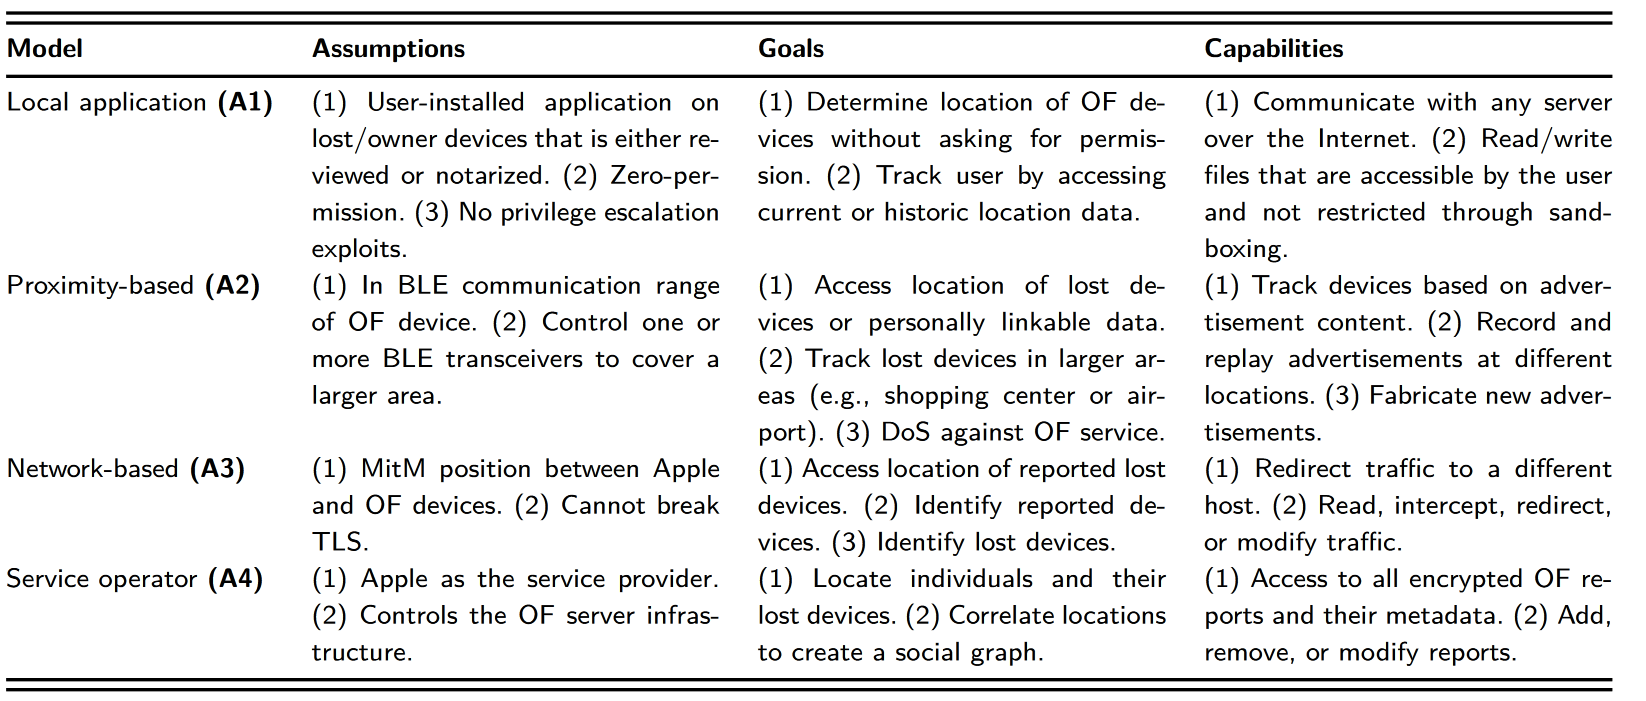
\includegraphics[width=\textwidth]{img/adversary_models}
  \caption{Angreifermodelle für den „Wo ist?“ Dienst \cite{Heinrich_FindMy}.}
  \label{fig:adversary_models}
\end{figure}

\autoref{tab:cia_adversary_models} ordnet den Zielen der einzelnen Angreifermodelle die betroffenen Sicherheitsziele zu.
\begin{table}[h]
  \caption{Zuordnung der Ziele der Angreifermodelle zu den allgemeinen Sicherheitszielen.}
  \label{tab:cia_adversary_models}
  \centering

  \begin{tabularx}{\textwidth}{ |l|X|X|l|X| }
    \hline
    \textbf{Angreifermodell}  & \textbf{Ziel} & \textbf{Vertraulichkeit} & \textbf{Integrität} & \textbf{Verfügbarkeit} \\
    \Xhline{0.5mm}
    \hline
    \multirow{2}{*}{A1} & (1) & \cmark & & \\
    \cline{2-5}
    & (2) & \cmark & & \\
    \hline
    \multirow{3}{*}{A2} & (1) & \cmark & & \\
    \cline{2-5}
    & (2) & \cmark & & \\
    \cline{2-5}
    & (3) & & (\cmark) & \cmark  \\
    \hline
    \multirow{3}{*}{A3} & (1) & \cmark & & \\
    \cline{2-5}
    & (2) & \cmark & & \\
    \cline{2-5}
    & (3) & \cmark & & \\
    \hline
    \multirow{2}{*}{A1} & (1) & \cmark & & \\
    \cline{2-5}
    & (2) & \cmark & & \\
    \hline
  \end{tabularx}
\end{table}
Dabei fällt auf, dass der Fokus auf der Vertraulichkeit der Daten liegt.
Bei der Erläuterung der Sicherheitsmaßnahmen im Folgenden wird deutlich, dass auch bei der Wahl von Maßnahmen durch Apple der Fokus auf der Vertraulichkeit liegt.
Somit ist davon auszugehen, dass beim Design des Dienstes ähnliche Angreifermodelle zugrunde gelegt wurden.
Sollten Angreifer Zugriff auf die Standortdaten erhalten, könnten sie diese für viele verschiedene Zwecke missbrauchen.
Zum Beispiel können diese Daten für gezielte Diskriminierung, Verfolgung und Überwachung durch Dritte oder auch durch staatliche Akteure verwendet werden.
Als personenbezogene Daten unterliegen die Standortdaten zusätzlich der \ac{DSGVO}.
Durch mögliche Rückschlüsse auf beispielsweise religiöse oder politische Überzeugungen sind Standortdaten nach Artikel 9 \ac{DSGVO} häufig auch als sensible personenbezogene Daten zu betrachten.
Deshalb ist Apple zumindest innerhalb der Europäischen Union auch verpflichtet, die Vertraulichkeit der Daten durch geeignete Maßnahmen zu schützen.
Wie bereits in \autoref{sec:Funktionsweise_FindMy} gezeigt, trifft Apple verschiedene Maßnahmen, die darauf abzielen die Vertraulichkeit zu wahren.
Die Auswirkungen dieser Maßnahmen werden in \autoref{sec:auswirkungen_sicherheitsmassnahmen} näher betrachtet.

Angriffe auf die Integrität und die Verfügbarkeit der Daten werden \cite{Heinrich_FindMy} nicht detailliert untersucht.
Nur das \textit{Proximity-based} Modell (A2 in \autoref{tab:cia_adversary_models}) zielt auch auf die Integrität und die Verfügbarkeit der Daten ab.
Wird die Verfügbarkeit beeinträchtigt, ist es für den Besitzer eines Geräts nicht mehr möglich, die aktuellen Standortdaten abzurufen.
Beide Sicherheitsziele sind hier eng miteinander verbunden.
Die Beeinträchtigung der Integrität durch Manipulation von Standortdaten führt beispielsweise dazu, dass der Besitzer nicht zwischen korrekten und manipulierten Daten unterscheiden kann.
Damit sind für den Besitzer keine zuverlässigen Standortdaten verfügbar.
Inwieweit Apples Sicherheitsmaßnahmen auch Integrität und Verfügbarkeit schützen, und welche Angriffe dennoch möglich sind, wird in \autoref{sec:auswirkungen_sicherheitsmassnahmen} und \autoref{sec:szenarien} näher betrachtet.
Außerdem wird in diesem Zusammenhang gezeigt, dass die von Heinrich \textit{et al.} \cite{Heinrich_FindMy} identifizierten Angreifermodelle nicht ausreichen, um alle hier aufgeführten Missbrauchsszenarien zu klassifizieren.

\subsection{Auswirkungen der Sicherheitsmaßnahmen}
\label{sec:auswirkungen_sicherheitsmassnahmen}

\subsubsection{Ende-zu-Ende Verschlüsselung}
Die Betrachtung der Funktionsweise in \autoref{sec:Funktionsweise_FindMy} zeigt, wie die Ende-zu-Ende-Verschlüsselung des Dienstes technisch umgesetzt wird.
Unter den Annahmen, dass ein Angreifer die Verschlüsselung nicht brechen kann und dass die Synchronisierung der \acp{MBK} über die iCloud-Keychain sicher ist, ist gewährleistet, dass nur der Besitzer des verlorenen Geräts dieses lokalisieren kann.
Auch wenn ein Angreifer direkt auf Apples Server zugreifen könnte oder die Daten auf dem Transportweg abgreifen könnte, sind die Standortinformationen der Lost Devices sicher.
Da die Entschlüsselung nur auf Owner Devices durch die sicher gespeicherten \acp{MBK} möglich ist, sind unverschlüsselte Standortinformationen niemals außerhalb eines Owner Devices verfügbar.
Als weitere Sicherheitsmaßnahme werden \ac{MITM}-Angriffe, bei der Kommunikation mit Apples Servern, durch die Verwendung von \ac{TLS}-verschlüsselten Verbindungen mit Certificate Pinning verhindert \cite{Heinrich_FindMy}.
Durch die Ende-zu-Ende-Verschlüsselung werden somit alle vom Netzwerkangreifer (A3 in \autoref{fig:adversary_models}) ausgehenden Bedrohungen adressiert.
Da lokale unprivilegierte Apps keinen Zugriff auf die in der iCloud-Keychain des Besitzers gespeicherten Schlüssel haben, werden so auch die von  lokalen Angreifern (A1 in \autoref{fig:adversary_models}) ausgehenden Bedrohungen behandelt.
Eine in \cite{Heinrich_FindMy} aufgedeckte Schwachstelle, die aufgrund von unsicherer Speicherung der Schlüssel unbefugten Zugriff auf die entschlüsselten Standortdaten ermöglichte, wurde durch Apple mittlerweile behoben.

Zusätzlich macht es die Ende-zu-Ende-Verschlüsselung auch Apple unmöglich, die Standortdaten der Nutzer zu entschlüsseln, womit das Lokalisieren durch den Dienstanbieter (Ziel (1) von A4 in \autoref{fig:adversary_models}) verhindert wird.
Außerdem verbessert die Verschlüsselung die Integrität der Daten, da einmal verschlüsselte Daten ohne Entschlüsselung nicht manipuliert werden können, ohne dass diese Manipulation erkannt werden kann.


\subsubsection{Schlüsselrotation}
Die Schlüsselrotation der Advertising Keys im Intervall von 15 Minuten bei Endgeräten und im Intervall von 24 Stunden bei Accesories, wie in \autoref{sec:Funktionsweise_FindMy} beschrieben, trägt ebenfalls zur Vertraulichkeit der Standortdaten bei.
Durch die regelmäßige Rotation der Schlüssel wird das Tracking von Geräten anhand der im Advertising gesendeten Daten erschwert.
Diese Maßnahme richtet sich gegen das Tracking durch einen Angreifer in der Nähe (A2 mit Ziel (2) in \autoref{fig:adversary_models}).
Außerdem müssten für einen solchen Angriff viele scannende Geräte so positioniert werden, dass auch bei Bewegung die Advertisement-Pakete des zu verfolgenden Geräts von einem der Scanner erfasst wird.
Um größere Bereiche abzudecken, wären jedoch sehr viele scannende Geräte notwendig, was den Angriff bereits deutlich erschwert.
In Verbindung mit der Schlüsselrotation ist die Verfolgung, auch mit hohem Aufwand, nur für das Intervall der Schlüsselrotation möglich.
Allerdings können AirTags und Drittanbieterprodukte durch das längere Intervall für bis zu 24 Stunden verfolgt werden.
Für Angreifer ist der Angriff jedoch insgesamt sehr aufwändig, sodass eine direkte Verfolgung des Opfers in den meisten Fällen praktikabler wäre.
Heinrich \textit{et al.} \cite{Heinrich_FindMy} betrachten die Schlüsselrotation als ausreichend, um die Verfolgung von Geräten nach diesem Muster zu verhindern.
Jedoch waren zum Zeitpunkt ihrer Analyse keine Geräte mit einem Intervall der Schlüsselrotation von mehr als 15 Minuten auf dem Markt.
Es ist unklar, ob die Autoren auch ein Rotationsintervall von 24 Stunden als ausreichend bewerten würden.


\subsection{Missbrauchsszenarien ohne ausreichende Gegenmaßnahmen}
\label{sec:szenarien}

Im Folgenden sind sechs Missbrauchsszenarien aufgeführt, welche nicht ausreichend durch Gegenmaßnahmen unterbunden werden.
Gegen einige werden gar keine Maßnahmen getroffen, andere Gegenmaßnahmen lassen sich leicht umgehen und sind dementsprechend nicht genügend.
Weiterhin beschreibt Szenario \nameref{missbrauch:4} sowohl einen negativen als auch einen positiven Missbrauch des Dienstes und ist deshalb differenziert zu betrachten.
Im einen Fall lässt sich der Dienst missbrauchen, um die Privatsphäre Dritter einzuschränken.
Im anderen Fall erfolgt der Missbrauch, zum besseren Schutz der Privatsphäre.
Weil dieser Anwendungsfall jedoch nicht von Apple vorgesehen ist, handelt es sich dennoch um Missbrauch.

Die folgenden Szenarien basieren auf den Arbeiten von Heinrich \textit{et al.} \cite{Heinrich_FindMy}, Tonetto \textit{et al.} \cite{Tonetto_FindMy}, Mayberry \textit{et al.} \cite{Mayberry_Tracking} und Garg \textit{et al.} \cite{Garg_Secure_Tracker}.

\subsubsection[M1]{M1: Replay-Angriff}
\label{missbrauch:1}
Durch die Ende-zu-Ende-Verschlüsselung und den authentifizierten Upload der Standortdaten, kann die Integrität der Standortdaten in vielen Fällen geschützt werden.
Allerdings können Replay-Angriffe genutzt werden, um dafür zu sorgen, dass manipulierte Standortdaten auf Apples Server und auf das Owner Device gelangen.
Diese sind korrekt verschlüsselt und werden ebenfalls korrekt authentifiziert hochgeladen, sodass für Apples Server keine triviale Möglichkeit besteht die Manipulation zu erkennen.

Durch Replay-Angriffe kann die Integrität der abgerufenen Standortdaten nicht mehr gewährleistet werden.
Der Nutzer kann bei abgerufenen widersprüchlichen Standortinformationen nicht zwischen korrekten und manipulierten Daten unterscheiden und erhält somit keine verlässlichen Standortinformationen, was die Verfügbarkeit beeinträchtigt \cite{Heinrich_FindMy}.
Dieser Angriff entspricht im wesentlichen \ac{DOS}-Angriff durch einen Angreifer in der Nähe (A2 mit Ziel (3) in \autoref{fig:adversary_models}).
Allerdings kann hier das Ziel auch in der reinen Manipulation der Standortdaten liegen, die Verfügbarkeit muss nicht in jedem Fall betroffen sein.
\begin{figure}[ht]
    \centering
    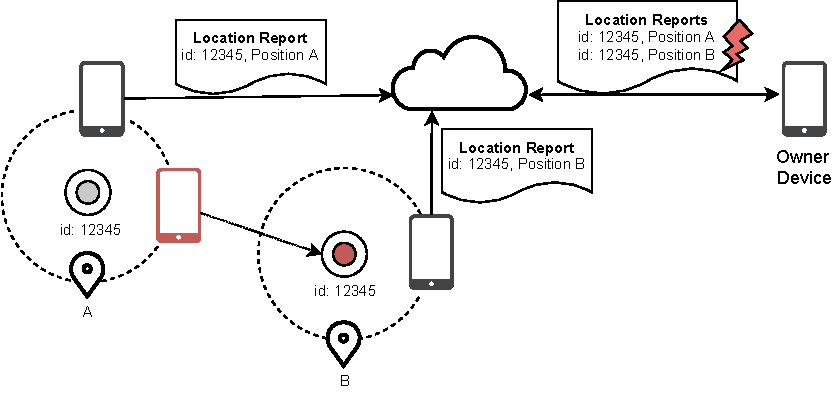
\includegraphics[width=0.9\textwidth]{replay.pdf}
    \caption{Schema eines Replay-Angriffs um die Integrität verfügbarer Standortdaten zu beeinträchtigen.}
    \label{fig:replay_attack}  
\end{figure}

Das grundsätzliche Schema eines Replay-Angriffs ist in \autoref{fig:replay_attack} dargestellt.
Um einen solchen Angriff durchzuführen, zeichnet ein Angreifer zunächst die Advertisement-Pakete und damit den öffentlichen Advertising Key eines Lost Device auf.
Anschließend kann der Angreifer die Aufzeichnung zu einer anderen Zeit oder an einem anderen Ort senden.
Geräte in der Nähe empfangen die wiederholten Pakete und erstellen Location Reports, welche mit dem enthaltenen Advertising Key verschlüsselt werden.
Bei einer Anfrage erhält das Owner Device beispielsweise sowohl korrekte als auch manipulierte Standortdaten.
Das Owner Device kann nicht bestimmen, welche Informationen korrekt sind und die Daten daher nicht für die Lokalisierung des Lost Device verwenden.

\subsubsection[M2]{M2: \ac{DOS}: Angreifer in der Nähe}
\label{missbrauch:2}
Die Verfügbarkeit der Standortdaten ist für die Betrachtung im Rahmen dieser Arbeit weniger relevant, da das Design des Dienstes vergleichsweise wenige Auswirkungen auf die Verfügbarkeit hat.
Dennoch ist die Verfügbarkeit durch verschiedene Angriffe bedroht.
Die Verfügbarkeit von Standortdaten lässt sich durch den Missbrauch von Funktionen des Dienstes durch einen Angreifer in \ac{BLE}-Reichweite eines Lost Device beeinträchtigen.
Dieser Angriff entspricht dem dritten Ziel des Angreifers in der Nähe (A3 mit Ziel (3) in \autoref{fig:adversary_models}).

Garg \textit{et al.} \cite{Garg_Secure_Tracker} zeigen bei einem von ihnen entwickelten Crowdsourced-Tracking Dienst, dass ein Angreifer in der \ac{BLE}-Reichweite des Geräts in der Lage ist, die Batterie des Geräts gezielt zu entladen.
Beim betroffenen System wird der aktuelle Standort vom Finder Device an das Lost Device gesendet, welches die Daten verschlüsselt zurückgibt.
Da sowohl Verschlüsselung als auch aktive \ac{BLE}-Kommunikation vergleichsweise energieintensiv sind, kann ein Angreifer durch das häufige Anfragen der Verschlüsselung die Batterie des Gerät entladen.

Ein Angriff nach diesem Schema kann prinzipiell auch Apples System betreffen.
Insbesondere für Accessories mit üblicherweise geringer Batteriekapazität ist die gezielte Entladung ein relevantes Bedrohungsszenario.
Da jedoch beim „Wo ist?“ Dienst die Verschlüsselung nicht auf dem Lost Device erfolgt, muss der Angriff leicht variiert werden.
Laut Apples Spezifikation müssen Accessories die Möglichkeit bieten, einen Ton abzuspielen.
Diese Funktion ist Teil der \ac{UT} und soll Nutzer vor direktem Tracking, wie in \nameref{missbrauch:3} beschrieben, warnen und das Auffinden versteckter Tracker ermöglichen \cite{Apple_FindMySpec}.
Allerdings kann diese Funktion durch alle Geräte in \ac{BLE}-Reichweite missbraucht werden, um Töne abzuspielen \cite{Heinrich_AirGuard}.
Das Abspielen von Tönen ließe sich im Rahmen eines Angriffes so lange wiederholen, bis die Batterie des Lost Devices entladen ist.

% Ein weiterer Angriff auf die Verfügbarkeit ist für Angreifer mit physischem Zugriff möglich.
% Durch Entfernen der Batterie oder Zerstörung des Accessories lässt sich die Verfügbarkeit der Standortdaten für den Besitzer des Geräts einschränken.
% Dies kann Angreifern, beispielsweise im Zusammenhang mit Diebstahl, helfen, die Auffindbarkeit gestohlener Gegenstände zu verringern.
% Allerdings stellt dieser Angriff keinen echten Missbrauch des „Wo ist?“ Dienstes dar, da keinerlei Funktionen des Dienstes genutzt werden.

\subsubsection[M3]{M3: Direktes Tracking von Personen}
\label{missbrauch:3}
Das Szenario des direkten Trackings von Personen bezieht sich auf die Verfolgung durch AirTags oder andere kleine Tracker.
Durch die kleine Größe der Tracker können diese in Jacken, Rucksäcken oder an Fahrzeugen befestigt werden, um einzelne Personen gezielt zu verfolgen \cite{Roth_airtags}.
Finder Devices in der Nähe der Tracker erzeugen Location Reports, die ein Angreifer zur Bestimmung der Position der Tracker und damit der Position des Opfers abrufen kann.
Solche Angriffe wurden bereits vielfach in der Praxis beobachtet und für Stalking oder Autodiebstahl genutzt \cite{NYT_Airtags}.
Dieses Szenario lässt sich keinem der Angreifermodelle von Heinrich \textit{et al.} \cite{Heinrich_FindMy} zuordnen, da es keinen Angriff auf den Dienst, sondern ein gezielter Missbrauch des Dienstes darstellt.
Der Angreifer ist ein legitimer Nutzer des Dienstes, der ein Lost Device lokalisiert.
Lediglich die Platzierung des Lost Devices unterscheidet diesen Angriff von einem normalen Einsatz des Dienstes.

Der „Wo ist?“ Dienst bietet zwar eine Funktion, um Nutzer auf mögliche Verfolgung hinzuweisen (\ac{UT}) \cite{Apple_FindMySpec}.
Diese ist nur für iOS automatisch verfügbar, sodass Android-Nutzer ohne eigenes Zutun nicht geschützt werden können.
Zusätzlich lässt sich die Funktion durch den Einsatz inoffizieller Tracker leicht umgehen und kann in vielen Fällen nicht zuverlässig vor Tracking warnen \cite{Heinrich_AirGuard,Mayberry_Tracking}.
Inoffiziell sind alle Tracker, welche den „Wo ist?“ Dienst ohne explizite Erlaubnis von Apple nutzen.
Solche Tracker lassen sich leicht aus kostengünstiger \ac{BLE}-Hardware und Open-Source-Software zusammenbauen und sind häufig günstiger als offizielle AirTags \cite{Heinrich_OpenHaystack,Mayberry_Tracking}.
Kennzeichen dieser Tracker ist die Möglichkeit, im Advertisement beliebige Daten zu senden, was genutzt werden kann, um die \ac{UT} zu umgehen \cite{Mayberry_Tracking}.

Da die Gegenmaßnahmen des „Wo ist?“ Dienstes gegen das direkte Tracking von Personen einfach umgangen werden können, sind sie als nicht ausreichend zu bewerten.
Wie genau die Gegenmaßnahmen umgangen werden können und welche Maßnahmen möglich sind, wird in \autoref{sec:gegenmassnahmen:3} beschrieben.


\subsubsection[M4]{M4: Indirektes Tracking von Personen}
\label{missbrauch:4}
Beim indirekten Tracking werden Personen nicht durch versteckte Tracker direkt verfolgt.
Stattdessen werden anhand der Uploadzeitpunkte von Location Reports Rückschlüsse auf die Bewegung von Personen gezogen.
Dieses Missbrauchsszenario wird von Tonetto \textit{et al.} in \cite{Tonetto_FindMy} vorgestellt und kann nicht nur für das schadhafte Tracking von Personen genutzt werden.
Stattdessen kann es auch zu Zwecken des Crowd-Monitorings genutzt werden und stellt dabei einen kleineren Eingriff in die Privatsphäre betroffener dar als alternative Methoden. 

Der Missbrauch beruht darauf, dass Location Reports generell gebündelt hochgeladen, und Apples Server den jeweiligen Uploadzeitpunkt mit einer Genauigkeit von wenigen Millisekunden speichern.
Damit können Angreifer Location Reports identifizieren, welche vom gleichen Finder Device stammen \cite{Tonetto_FindMy}.
Während Finder Devices mit Mobilfunkverbindung Location Reports in der Regel erst nach einigen Stunden hochladen, erfolgt der Upload bei einer WLAN-Verbindung deutlich schneller.
Wechselt ein Finder Device von einer Mobilfunkverbindung zu einer WLAN-Verbindung, werden die zwischengespeicherten Location Reports in der Regel kurz darauf hochgeladen.
Unter der Annahme, dass Personen außerhalb einiger weniger Orte, wie zum Beispiel der eigenen Wohnung, nicht dauerhaft mit einem WLAN-Netzwerk verbunden sind, werden außerhalb dieser Orte erstellte Location Reports in etwa zur gleichen Zeit hochgeladen \cite{Tonetto_FindMy}.
Auch dieses Szenario lässt sich keinem der Angreifermodelle zuordnen. 
Der Angreifer ist im Wesentlichen ein legitimer Nutzer des Dienstes, der lediglich die vom Dienst bereitgestellten Daten in anderer Weise auswertet.
Um die Location Reports zu erhalten, muss die \ac{API} des Dienstes direkt genutzt werden anstatt die offizielle „Wo ist?“ App zu nutzen, die nur die Standorte anzeigen kann.
Ansonsten wird der Dienst wie vorgesehen genutzt \cite{Tonetto_FindMy}.

\autoref{fig:indirect_tracking} zeigt ein Beispiel für das indirekte Tracking von Personen.
Ein Angreifer platziert mehrere Tracker an verschiedenen Orten.
Im hier gezeigten Beispiel werden zwei Tracker mit jeweils festem Advertising Key, vereinfacht als \textit{id} dargestellt verwendet.
Finder Devices in der Nähe erfassen die Tracker und erstellen Location Reports.
Der Angreifer kann die Location Reports, die sich auf seine Tracker beziehen, herunterladen und erhält dabei auch die Uploadzeitpunkte.
Mehrere Location Reports mit gleichem Uploadzeitpunkt stammen mit hoher Wahrscheinlichkeit vom gleichen Finder Device, sodass der Angreifer die Reports nach Finder Devices gruppieren kann.
Im Beispiel können die ersten beiden heruntergeladenen Location Reports anhand der gleichen Uploadzeit (\textbf{54321}) dem Opfer zugeordnet werden.
Die Reports enthalten neben dem Uploadzeitpunkt auch den Zeitpunkt der Erstellung und können somit auch nach der Erstellungszeit geordnet werden.
Dadurch kann der Angreifer den Pfad, den das Opfer zurückgelegt hat, rekonstruieren.
Mit steigender Anzahl eingesetzter Tracker, steigt auch die Genauigkeit der rekonstruierten Pfade.
\begin{figure}[ht]
  \centering
  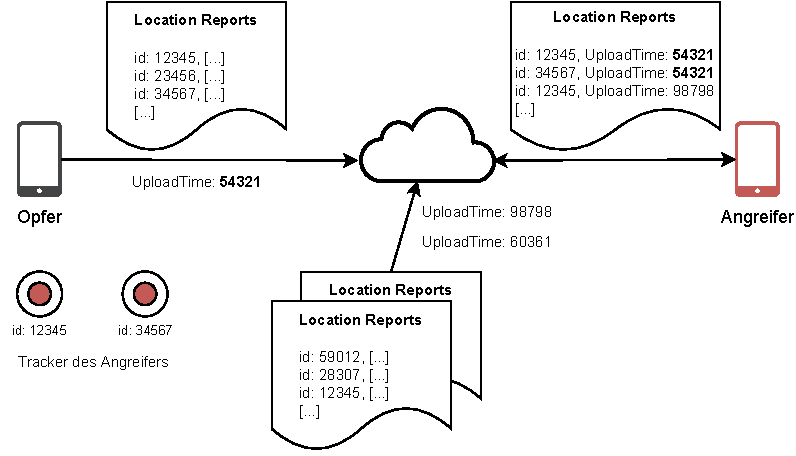
\includegraphics[width=0.9\textwidth]{indirektes_tracking.pdf}
  \caption{Schema zum indirekten Tracking von Personen.}
  \label{fig:indirect_tracking}
\end{figure}

Zur Nutzung als Tool für das Crowd-Monitoring werden einzelne Tracker an öffentlichen Orten platziert.
Finder Devices, die sich in der Nähe dieser Tracker befinden, generieren Location Reports und laden diese hoch.
Diese Reports können von Apples Servern heruntergeladen werden und erlauben Rückschlüsse über die Anzahl der iPhone-Nutzer, welche sich zu einem bestimmten Zeitpunkt in der Nähe eines Ortes aufgehalten haben.
Dazu werden die Erstellungszeitpunkte der Reports und die Anzahl der Reports für einen bestimmten Tracker herangezogen.
Die Zahl der iPhone-Nutzer kann weiterhin verwendet werden, um die Gesamtzahl der Personen zu schätzen.
Durch die Verzögerung beim Upload der Reports sind die Daten allerdings nur mit einer gewissen Verzögerung verfügbar \cite{Tonetto_FindMy}.

Über die Verwendung mehrerer Tracker lassen sich weiterhin die Bewegungen von Menschenmengen, der sogenannte Crowd-Flow, rekonstruieren.
Dabei werden die Tracker an verschiedenen Orten platziert und die Location Reports der Finder Devices heruntergeladen.
Anhand der Uploadzeitpunkte der Reports kann bestimmt werden, welche Reports vom gleichen Finder Device stammen \cite{Tonetto_FindMy}.
Darauf aufbauend kann die Zeit bestimmt werden, die das Finder Device benötigt hat, die Distanz zwischen jeweils zwei Trackern zurückzulegen.
Alternativ könnte, über das oben vorgestellte Verfahren, die Anzahl der Personen in der Nähe jedes Trackers zu verschiedenen Zeiten bestimmt werden und auf Basis der Veränderungen Rückschlüsse auf die Bewegungen der Menschenmengen gezogen werden.


Dieser Missbrauch des „Wo ist?“ Dienstes kann als Alternative zu aktuellen Crowd-Monitoring-Systemen, welche auf Bilderkennung oder der Auswertung von Wi-Fi Management Frames basieren, verwendet werden und erlaubt eine ähnliche Genauigkeit bei geringerem Eingriff in die Privatsphäre der betroffenen Personen.
Zusätzlich ist dieser Ansatz besser für die Privatsphäre der Betroffenen, da keine personenbezogenen Daten erhoben werden \cite{Tonetto_FindMy}.
Deshalb wird dieser Einsatzzweck als „positiver“ Missbrauch des „Wo ist?“ Dienstes bewertet.

\subsection[M5]{M5: Verdeckter Datentransfer}
\label{missbrauch:5}
Tonetto \textit{et al.} \cite{Tonetto_FindMy} und Bräunlein \cite{braeunlein_sendmy} zeigen unabhängig voneinander, dass der „Wo ist?“ Dienst auch für einen verdeckten Datentransfer mit einer niedrigen Übertragungsrate ausgenutzt werden kann.
Dabei werden Finder Devices dazu genutzt, Daten an Apples Server zu übertragen, welche vom Angreifer heruntergeladen und dekodiert werden können.
Beide verwenden für das Senden der Daten inoffizielle Tracker, um die Daten in den Advertisements zu senden.
Der verdeckte Datentransfer kann dem Angreifermodell des Angreifers in der Nähe (A2 in \autoref{fig:adversary_models}) zugeordnet werden.
Allerdings muss das Angreifermodell um das Ziel eines kostenfreien und unentdeckten Datentransfers und der Möglichkeit die Location Reports über die \acp{API} des Diensts herunterzuladen erweitert werden.


Bräunlein \cite{braeunlein_sendmy} kodiert eine zu sendende Nachricht in den öffentlichen Schlüssel, der in Advertisement-Paketen übertragen wird.
Für jedes Bit der Nachricht wird ein 28 Byte langes Array, bestehend aus der Position des Bits in der Nachricht, einer ID des Senders und dem Wert des Bits generiert.
Anstatt einen öffentlichen Schlüssel im Advertisement zu senden, werden die so kodierten Daten für eine definierte Zeitspanne gesendet.
Danach wird der Prozess für das nächste Bit der Nachricht wiederholt.
Diese Kodierung ist in \autoref{fig:sendmy_encoding} schematisch dargestellt.
\begin{figure}[ht]
  \centering
  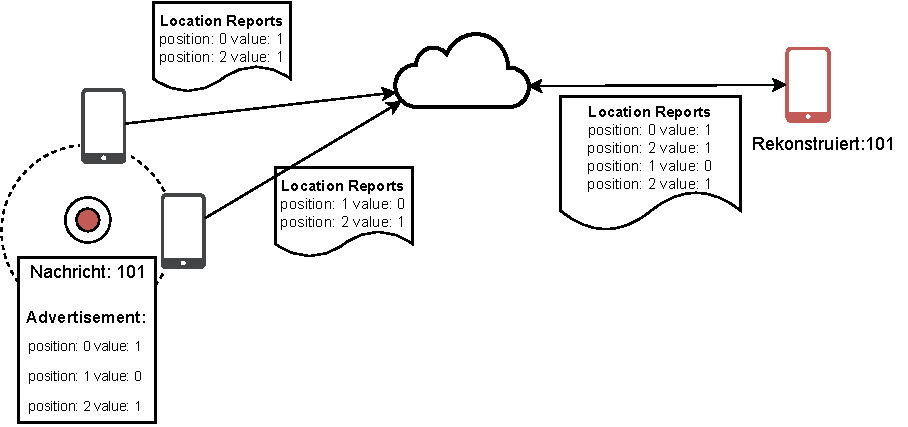
\includegraphics[width=0.95\textwidth]{sendmy.pdf}
  \caption{Bitweise Kodierung einer Nachricht in Advertisement-Pakete, wie von Bräunlein vorgeschlagen.}
  \label{fig:sendmy_encoding}
\end{figure}
Der Empfänger kann für jedes Bit der Nachricht die zwei möglichen Arrays generieren und eine Anfrage mit den jeweiligen \ac{SHA}-256 Hashes an Apples Server senden.
Da jedoch nur ein öffentlicher Schlüssel erzeugt wird, können mit diesen Schlüsseln verschlüsselte Nachrichten nicht entschlüsselt werden.
Jedoch ist für diesen Missbrauch die Entschlüsselung der Daten nicht notwendig, da lediglich das Vorhandensein eines bestimmten Location Reports überprüft werden muss, um die Nachricht zu dekodieren.
Abhängig davon, welcher der beiden Hashes in der Antwort enthalten ist, kann der Empfänger das Bit der Nachricht bestimmen.
Dabei wird ausgenutzt, dass jedes Apple Gerät die verschlüsselten Location Reports für beliebige öffentliche Schlüssel herunterladen kann \cite{Heinrich_OpenHaystack,braeunlein_sendmy}.
Da die Location Reports Ende-zu-Ende verschlüsselt sind, wird dadurch die Vertraulichkeit nicht gefährdet.
Ein Nachteil bei diesem Verfahren ist, dass somit theoretisch jedes Apple-Gerät die Nachricht abrufen könnte.

\begin{figure}[ht]
  \centering
  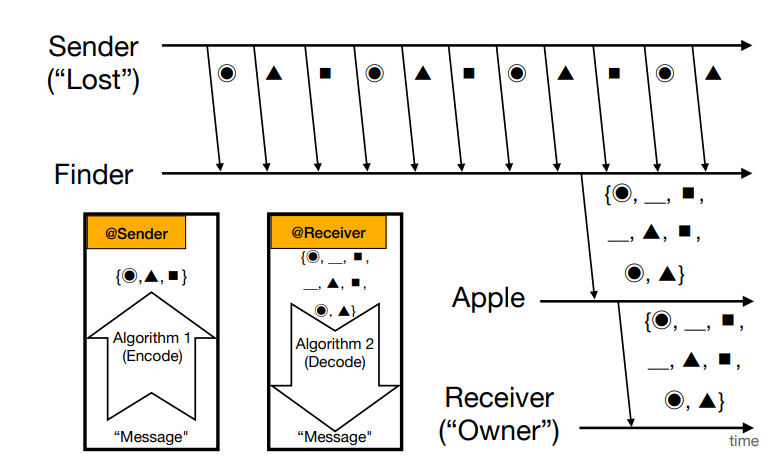
\includegraphics[width=0.7\textwidth]{tagcomm.png}
  \caption{Kodierung einer Nachricht in eine Folge bekannter Advertising Keys, wie von Tonetto \textit{et al.} vorgeschlagen \cite{Tonetto_FindMy}.}
  \label{fig:tagcomm_encoding}
\end{figure}
Das von Tonetto \textit{et al.} \cite{Tonetto_FindMy} vorgestellte Verfahren verwendet stattdessen 16 bekannte Advertising Keys, um die Nachricht in eine Folge dieser Keys zu kodieren.
Dazu wird eine Menge von Advertising Keys zuvor generiert und zwischen Sender und Empfänger ausgetauscht.
Das Verfahren ist in \autoref{fig:tagcomm_encoding} schematisch dargestellt.
Zunächst erzeugt der Sender aus der Nachricht eine Abfolge der Advertising Keys.
Diese werden in dieser Reihenfolge nacheinander in den Advertisement-Paketen gesendet.
Finder Devices, die sich in der Nähe befinden, empfangen die Advertisement-Pakete, erstellen Location Reports und laden diese hoch.
Der Empfänger der Nachricht kann alle Location Reports der bekannten Advertising Keys herunterladen.
Da der Empfänger die Location Reports entschlüsseln kann, erhält er die Zeitstempel der Erstellung der Location Reports.
Daraus kann er die Folge der Advertising Keys rekonstruieren und die Nachricht dekodieren.

Im Vergleich zum Verfahren von Bräunlein, werden hier echte Advertising Keys verwendet, sodass die Location Reports entschlüsselt werden können, sodass der Standort des Senders bestimmt werden kann.
Zusätzlich muss der Empfänger weniger Anfragen an Apples Server stellen, da nur 16 unterschiedliche Advertising Keys verwendet werden.
Bräunleins Verfahren benötigt hingegen zwei Anfragen an Apples Server pro übertragenem Bit \cite{braeunlein_sendmy}.


\subsection[M6]{M6: Korrelation von Standorten durch Apple}
\label{missbrauch:6}

Das zweite Ziel im Angreifermodell des Dienstanbieters (A4 in \autoref{fig:adversary_models}) bezieht sich auf die Korrelation von Standorten mehrerer Nutzer.
Heinrich \textit{et al.} \cite{Heinrich_FindMy} zeigen, dass durch den authentifizierten Upload und Download, die Korrelation durch Apple theoretisch möglich ist.
Die konkreten Standorte können aufgrund der Ende-zu-Ende-Verschlüsselung nicht bestimmt werden.
Allerdings kann bestimmt werden, welches Gerät welche Location Reports erstellt und welcher Nutzer diese heruntergeladen hat.
Daraus lässt sich folgern, welche Nutzer sich zu welcher Zeit an einem gemeinsamen Ort aufgehalten haben.
Apple könnte diese Informationen für eigene Zwecke nutzen, zum Beispiel um soziale Beziehungen zwischen Nutzern für personalisierte Werbung zu analysieren.
In \cite{Heinrich_FindMy} wird zusätzlich gezeigt, dass diese Daten auch von Strafverfolgungsbehörden genutzt werden könnten, um beispielsweise die Identität von Demonstrationsteilnehmern zu bestimmen.

Zumindest nach US-Recht existieren verschiedene Möglichkeiten für Strafverfolgungsbehörden, von Apple gespeicherte Daten anzufragen \cite{Data_Access}.
In den „Richtlinien für Rechtsverfahren [für] Regierungs- und Strafverfolgungsbehörden außerhalb der USA“ \cite{Apple_FindMy_Data} gibt Apple an, dass aufgrund der Verschlüsselung kein Zugriff auf die Standortdaten der Nutzer möglich ist.
Allerdings stehen „Verbindungsprotokolle zu ‚Wo ist?’ [stehen] für einen Zeitraum von bis zu 25 Tagen zur Verfügung“ \cite{Apple_FindMy_Data}.
Um diese Verbindungsprotokolle zu erstellen, muss eine Zuordnung von Verbindungen zu Nutzern stattfinden.
Da Verbindungen zum „Wo ist?“ Dienst nur beim Upload oder Download von Location Reports entstehen, kann davon ausgegangen werden, dass Apple diese Daten speichert.
Mit den Daten zur Authentifizierung kann Apple alle Location Report zu bestimmten Nutzern zuordnen.
Das hier beschriebene Szenario ist dadurch auch praktisch umsetzbar und könnte bei entsprechendem Zugriff nicht nur von Apple, sondern auch von Strafverfolgungsbehörden genutzt werden.



% \subsection{Zusammenfassung Missbrauchsszenarien ohne ausreichende Gegenmaßnahmen}
% In \autoref{tab:missbrauchsszenarien} werden die Missbrauchsszenarien zusammengefasst, gegen welche von Apple aktuell keine ausreichenden Gegenmaßnahmen ergriffen werden.
% Dazu sind die Zielsetzung des Angreifers und mögliche Betroffene eines solchen Angriffs aufgeführt

% \begin{table}[ht]
%   \caption{Zusammenfassung der Missbrauchsszenarien \nameref{missbrauch:1} bis \nameref{missbrauch:6}.}
%   \label{tab:missbrauchsszenarien}
%   \begin{tabularx}{\textwidth}{ |l|X|X|X| }
%     \hline
%     \textbf{Szenario} & \textbf{Beschreibung} & \textbf{Angriffsziel} & \textbf{Betroffene}\\
%     \Xhline{0.5mm}
%     \hline
%     \nameref{missbrauch:1} & Replay-Angriff & Integrität, Verfügbarkeit & Nutzer des „Wo ist?“ Dienstes \\
%     \hline
%     \nameref{missbrauch:2} & \ac{DOS}: Angreifer in der Nähe & Verfügbarkeit & Nutzer des „Wo ist?“ Dienstes \\
%     \hline
%     \nameref{missbrauch:3} & Direktes Tracking & Vertraulichkeit & Jeder \\
%     \hline
%     \nameref{missbrauch:4} & Indirektes Tracking & Vertraulichkeit & Nutzer des „Wo ist?“ Dienstes  \\
%     \hline
%     \nameref{missbrauch:5} & Verdeckter Datentransfer & Ausnutzung zur Datenübertragung & Apple \\
%     \hline
%     \nameref{missbrauch:6} & Korrelation von Nutzerstandorten & Vertraulichkeit & Nutzer des „Wo ist?“ Dienstes \\
%     \hline
%   \end{tabularx}
% \end{table}
